\documentclass{jsarticle}

% パッケージ
\usepackage[dvipdfmx]{graphicx}
\usepackage{url}
\usepackage{amsmath}


\begin{document}

% 脚注フォーマット
\renewcommand\thefootnote{\arabic{footnote})}


% 表紙

{\Large \today 提出}\\ % 提出日

\begin{center}
\vspace{120truept}
{\huge 平成29年度 卒業論文\\[10mm]
日本のIPO市場における\\アンダープライシングの時系列分析}\\ % タイトル
\vspace{120truept}
{\huge 岡部 匡志\\
\vspace{50truept}
東京大学経済学部経済学科\\
\vspace{50truept}
07-150041}\\ % 著者

\end{center}
\newpage
\begin{center}
{\Large 日本のIPO市場におけるアンダープライシングの時系列分析}\\ % タイトル
\end{center}

% 目次
\tableofcontents

\vspace{50truept}
% 本文
\section{はじめに}
本稿では、日本の新規株式公開\footnote[1]{Initial Public Offering。以下、 「IPO」とする。}市場において、アンダープライシング\footnote[2]{\{(初値) - (公開価格)\} / (公開価格) として示される。初期収益率とも。100\%からの乖離を、初期乖離率と呼ぶこともある。ここで、公開価格とは、「IPO直前に希望する投資家に対して新規公開予定の株式を売却する際の価格(岡村 2011\cite{okamura})である。また、本稿では初値として、マーケットで付けられた、取引初日における最初の価格を用いる。}の過去数件の値が、当期のアンダープライシングににどのような影響を及ぼしているのかについて考察を行う。\par
著者の知る限り、アンダープライシングの研究において、その系列相関をモデルに積極的に引き受けた研究は見当たらない。そのため、実証分析の対象が、5年程度と比較的短い期間であったり、年度ダミーを説明変数に入れて、年度ごとのマーケットの過熱度を表現している研究が多い印象である。\par
本稿では、年度ダミーではなく、自己回帰モデルを用いることで、20年間の長期に渡ってマーケット・コンディションを表現可能なモデルを構築する。\par
本稿の構成は以下の通りである。次章で、日本のIPOマーケットと、アンダープライシングの発生メカニズムをめぐる仮説を概観する。第3章では、本稿で検証する仮説を提示し、その検証方法と用いるデータについて説明する。第4章で実証分析で得られた結果について考察し、第5章で総括と今後の課題について言及する。

\newpage
\section{IPOにおけるアンダープライシング}

\subsection{IPOのプレイヤーとメカニズム}
本題に入る前に、我が国におけるIPOのメカニズムについて、簡単に説明しておこう。\par
IPOにおける主要なプレーヤーは、新規公開企業(公開会社)、アンダーライター\footnote[3]{ここでは、株式の発行・売出しに際し、株式を売れ残った際に発行者や所有者から取得する者のことであり、日本国内においては、IPOを主導する主幹事証券会社を中心としたシンジゲート団のことを指す。}、投資家の3者に分けられる。\par
公開会社、およびその既存株主が、新規に株式を公開するにあたり、まずアンダーライターを通して、国内の一般投資家を中心に、「公開価格」で株式が販売される\footnote[4]{一般に、「公募」と呼ばれる新株式の発行と、「売出し」と呼ばれる既存株主による売却が同時に実施される。また、ブックビルディング時に想定以上の需要があった場合、既存株主から株式を一時的に借りて販売する「オーバーアロットメント」も制度化されている。}。アンダーライターによって配分方法は異なるが、7割から9割が個人投資家への配分となっているようである。\par
上場日\footnote[5]{公開価格が決定してから8営業日程度前と言われる。}になると、公開会社ごとに定められた証券市場で、公開会社の株式が取引可能になる。そこで、取引初日に初めて成立した売買における価格が「初値」である。\par
公開価格は、1997年以降\footnote[6]{以前は公開価格が高くなりがちな、入札方式しか認められていなかった。本稿で扱うサンプル・データは全てブックビルディング方式で公開価格が決められている。}、ブックビルディング方式で決定されている。ブックビルディング方式とは、まず、株価算定能力が高いと思われる機関投資家へのヒアリングを元に、仮条件価格帯を決定する。その仮条件価格帯内における、投資家の需要状況を把握し、公開価格を決定する、というものである。一般投資家が公開価格で株式を購入するためには、このブックビルディングに参加しなければならない。公開価格以上で発注した投資家に、購入申し込みの権利が与えられる。\\ \par
さて、前述したとおり、アンダープライシングは次式で与えられる。

\begin{equation}
Underpricing = \frac{P_{open} - P_{book}}{P_{book}} \nonumber
\end{equation}
\par
ここで、$P_{open}$は初値、$P_{book}$は公開価格である。


\subsection{アノマリーとしてのアンダープライシング}
表\ref{around_world}に示すように、アンダープライシングの期待値が継続的に100\%を上回る値を取ることは、国内外において確認されており、一種の経済学的アノマリー\footnote[7]{例えば、辰巳・桂山 2005\cite{tatsumi}が、ファイナンス分野で知られるアノマリーに詳しい。}として知られている。 \par
公開価格には企業のファンダメンタルズが適切に評価されており、初値は株式市場において効率的に形成されると想定するなら、このような現象が放置されている事実は、やはり、アノマリーと言えるだろう。\par

\begin{table}[h]
	\caption{世界各国における初期収益率の算術平均。
	Loughran et el.(1994, updated 2015) \cite{Loughran}より一部抜粋。}
	\label{around_world}
	\centering
	\begin{tabular}{cccc}
		\hline
		国名&サンプル数&期間&平均初期収益率(100\%からの乖離) \\
		\hline \hline
		英国&4,932&1959-2012&16.0\% \\
		韓国&1,758&1980-2014& 58.8\% \\
		シンガポール&609&1973-2013&25.8\% \\
		タイ&500&1987-2012&35.1\%\\
		台湾 &1,620 &1980-2013&38.1\% \\
		中国&2,512&1990-2013&118.4\%\\
		ドイツ&736&1978-2011&24.2\% \\
		日本&3,236&1970-2013&41.7\% \\
		フランス & 697 & 1983-2010 & 10.5\% \\
		米国&12,702&1960-2012&16.9\%\\
		\hline
	\end{tabular}
	\end{table}
	 \par

この状況の下では、投資家は、公開価格で株式を購入し、数週間後の上場後に株式を売却するだけで、高いリターンを得られる。実際、ブックビルディングにおける株式購入には、投資家からの注文が殺到し、抽選が行われるのが通例である。\par
また、公開会社にとっては、$P_{open}$と$P_{book}$の差額は、資金調達における機会損失を意味する。 \\ \par
この、株式市場における、ある種の裁定取引の機会は、いったいどのように説明されるのだろうか?





\subsection{アンダープライシングをめぐる仮説}
アンダープライシングは、IPOにおけるアノマリーとして、研究者や投資家たちの強い関心を集めてきた。特に研究面の関心は、アンダープライシングを合理的に説明する決定メカニズムの解明に向けられており、現在に至るまで数多くの仮説が提案されている。\par
既存研究における、アンダープライシングの決定メカニズムをめぐる仮説は、大きく2つに分類出来る。すなわち、アノマリーの原因を情報の非対称性や、観測不能性に求めるものと、各プレーヤーの限定合理性に求めるものである。\\ \par
前者の仮説については、岡村 2011\cite{okamura}によく整理されている。本稿では名前を列挙するに留めるが、「逆選択回避仮説(別名:Winner's Curse)」「エージェンシー仮説」「情報顕示仮説」「利益相反仮説」など、それぞれ、アンダーライターが公開価格を引き下げる誘引を持つことを説明している。\par

また、アンダーライターではなく、投資家の側に、ブックビルディングにおける需要の申告に際して、株式の市場価格の観察不能性によるリスクの存在から、公開価格を押し下げる誘引が存在することを説明した研究として、池田 (2013)\cite{ikeda}がある。\\ \par

一方で、近年の行動経済学・行動ファイナンスの発展に伴い、プレーヤーの限定合理性を導入してアンダープライシングを説明しようとする研究が展開されている。その代表的なものとして、「後の投資家は、それまでの他の投資家が行った購入意思決定を意思決定に反映させ、自らの都合に合わせて情報を無視、あるいは軽視し、先の投資家に追随する」という、いわゆる情報カスケード効果\footnote[8]{Welch (1992)\cite{Welch}がその端緒とされている。}が挙げられるだろう。\\ \par



現実的な解釈としては、「どの仮説が正しい/誤っている」という問題ではなく、それぞれの仮説が折り重なって実際のアンダープライシングが形成されている、ということになる。以下、本稿では、図\ref{transition}のように、アンダープライシングの程度が時期によって大きく異なっていることに注目し、情報カスケード効果を想定した、マーケット・コンディションの存在と、その解明について論じていく。

\begin{figure}[t]
  \begin{center}
  \caption{アンダープライシングの年度別平均値の推移(1997〜2016) 後述のデータより著者作成(以下同様)。}
    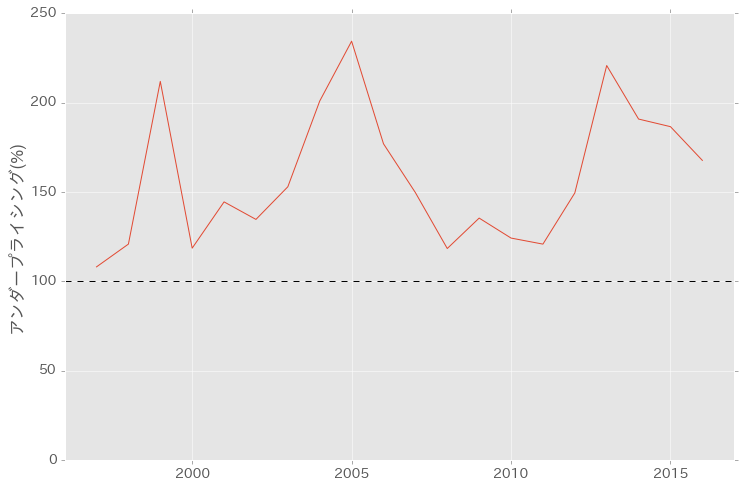
\includegraphics[clip,width=14cm]{./transition.png}
    \label{transition}
  \end{center}
\end{figure}


\section{リサーチ・デザイン}
\subsection{本研究の目的と意義}
金子 (2009)\cite{kaneko}も指摘する通り、「間もなく発行される株式をいくら以下なら購入してもよいかを考える際に、投資家がおそらくもっとも参考にしたいと考える現在の株価が、PO(著者注:すでに株式を公開している企業が一般投資家向けに株式を発行すること)の方は存在するがIPOの方は存在しない」(p.84)ことが、IPOの初値形成における固有の事情と言える。\\ \par
それでは、投資家は何を参考に、情報が不足する株式の購入意思決定を行っているのだろうか?\\ \par
本稿では、$Underpricing$の過去数件の値が、当期のIPOの$Underpricing$に影響を与えると考える。すなわち、直近のIPOにおいて高い$Underpricing$が観測されたとき、投資家は自分が持つ、当該企業についてのファンダメンタルズの情報を軽視し、「今はマーケット・コンディションが良い」と考えることで、高い$P_{open}$を付けるのではないか、という仮説である。\\ \par
同時に、ここで、マーケット・コンディションとは、経済一般における「景気」とは独立した指標であり、通常の株式市場における価格の上下とは無関係に動く、ということも主張したい。\\ \par

独自のマーケット・コンディション指数を定義し、$Underpricing$への回帰を行った研究として、Derrien (2005)\cite{Derrien}が挙げられる。Derrienは、マーケット・コンディションを、IPO企業の属する業種インデックスの上場前3ヶ月間のパフォーマンスと定義している。本稿では、マーケット・コンディション指数を積極的に設定することはせず、当該企業のIPO時における直近の数件のIPOパフォーマンスそれ自体が、マーケット・コンディションとして機能していると考える。\\ \par


著者の知る限りにおいて、アンダープライシングの研究において、その系列相関をモデルに積極的に引き受けた研究は見当たらない。そのため、実証分析の対象が、5年程度と比較的短い期間であったり、年度ダミーを説明変数に入れて、年度ごとのマーケットの過熱度を表現している研究が多い印象である。\par
本稿は、年度ダミーではなく、自己回帰モデルを用いることで、20年間の長期に渡ってマーケット・コンディションを表現可能なモデルを構築しようとするものである。

\subsection{データ・ソース}
前章で提示した、「直近のIPOのパフォーマンスが、当該IPOのパフォーマンスに影響を与える」という仮説を検証するために、1997年9月に上場した株式会社フォトロン(現:株式会社イマジカ・ロボット ホールディングス)から、2016年12月に上場した株式会社グッドコムアセットまでの、計1962社をサンプル・データとして用いる\footnote[9]{データは、\url{https://github.com/M-okb/IPO_analysis}で公開している。用いたデータの内、1997年から2009年のものについては、Kaneko and Pettway’s Japanese IPO Database(\url{http://www.fbc.keio.ac.jp/~kaneko/KP-JIPO/top.htm})で公開されているデータから、2010年以降のものについては、総合投資情報サイト(\url{http://www.traders.co.jp/})、Yahoo finance(\url{http://stocks.finance.yahoo.co.jp/})から取得した。ここに感謝の意を表します。}。\par
なお、上場中止・上場延期になったもの(例:株式会社ZMP)や、J-REIT(例:星野リゾート・リート投資法人)などは扱っていない。\par

\subsection{データの特徴}
\subsubsection{アンダープライシング}
前述したとおり、図\ref{transition}のように、年度によってアンダープライシングの度合いは大きく異なる。具体的には、2000年\footnote[10]{IPOバブル崩壊の年である。政府による起業支援や、ストック・オプションの規制緩和などを受け、WEB関連銘柄を中心に市況が活性化したが、2000年3月の光通信の不正をきっかけに、WEB関連銘柄の株価は大きく値下げした。}前後で大きく下落している他、2005年がピークとなっており、2010年周辺では100\%は割らないとは言え、低迷していることが分かる。\par
全てのアンダープライシングをヒストグラムに取ったのが図\ref{hist}であり、値は正規分布せず、右に裾野の広い分布となっている。
図\ref{loghist}に、それを対数表示した。既存研究では、アンダープライシングを百分率で表示し、それを被説明変数に用いることが多かったが、本稿では百分率でなく、比率を自然対数で表示したものを用いる。\par

\newpage

\begin{figure}[!h]
  \begin{center}
  \caption{アンダープライシング(1997〜2016)の分布ヒストグラム}
    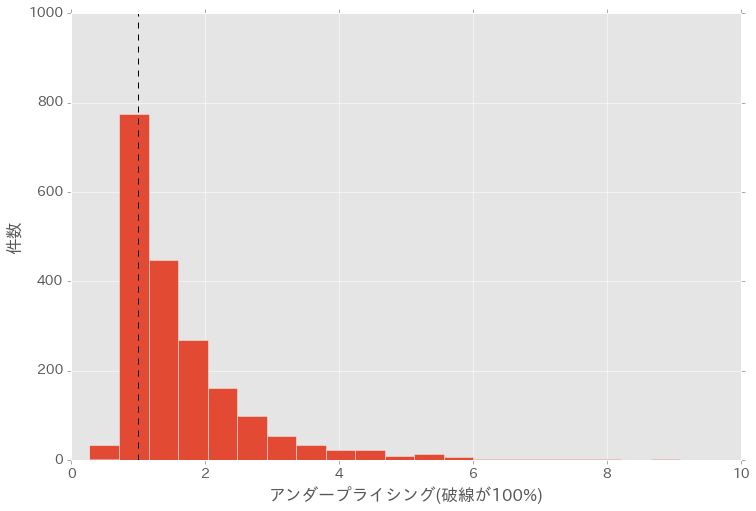
\includegraphics[clip,width=14cm]{./hist.png}
    \label{hist}
  \end{center}
\end{figure}

\begin{figure}[!h]
  \begin{center}
  \caption{アンダープライシング(1997〜2016)の対数分布ヒストグラム}
    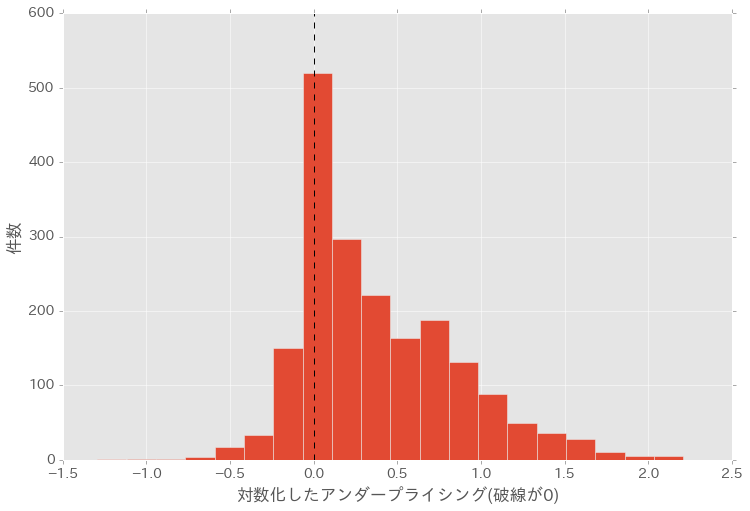
\includegraphics[clip,width=14cm]{./loghist.png}
    \label{loghist}
  \end{center}
\end{figure}

\newpage



\begin{table}[t]
  \begin{center}
  \caption{アンダープライシングの基本統計量の5年おきの推移(1997〜2016)}
\begin{tabular*}{120mm}{@{\extracolsep{\fill}}c|ccccc}

\hline
\  & 総計 &  1997 &  2002&   2007  & 2012 \\
\hline \hline
件数 &1962 & 606 & 766 & 249 & 341 \\
\hline
標準偏差&       0.990  &0.911  &1.080 & 0.601 & 1.005 \\
\hline
平均値   &  1.647 & 1.417 & 1.836 & 1.357 & 1.840 \\
\hline
最小値    &     0.275 & 0.275 & 0.583 & 0.571&  0.531 \\
25\%tile   &       1.026 & 1.000  &1.094 & 0.941 & 1.089 \\
50\%tile    &      1.271&  1.115 & 1.472 & 1.077  &1.486 \\
75\%tile     &     1.999 & 1.500 & 2.183  &1.694 & 2.294 \\
最大値  &   9.091 & 9.091&  8.727 & 4.086 & 5.625 \\
\hline
	\end{tabular*}
	\label{stats} 
  \end{center}
\end{table}

アンダープライシングの5年おきの基本統計量の推移を表\ref{stats}に示した。どの時代でも、おおよそ、25\%tileを境目として、アンダープライシングがプラスとなることが分かる。\par

\subsubsection{IPO件数}
年度別のIPO数は図\ref{fig:year}のようになっており、多い年では、少ない年の10倍近くのIPOがある。こちらは、アンダープライシングとは異なり、IPOバブル崩壊の影響は限定的であるが、2008年のリーマン・ショックの影響を大きく受けているように見受けられる。



\begin{figure}[t]
  \begin{center}
  \caption{IPO数の年度別推移(1997〜2016)}
  \begin{tabular}{c}
  \begin{minipage}{0.5\hsize}
  \begin{center}
    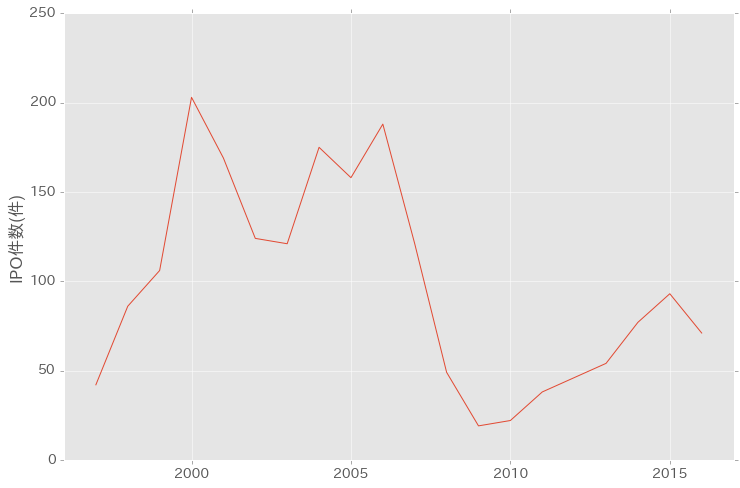
\includegraphics[clip,width=9cm]{./year_count.png}
     \end{center}
\end{minipage}
\begin{minipage}{0.5\hsize}
\begin{center}
    \label{fig:year}
\begin{tabular}{cc|cc}
		\hline
		年度 & 件数 & 年度 & 件数 \\
		\hline \hline
1997  &   42 & 2007  &  121\\
1998  &   86 & 2008   &  49\\
1999   & 106 & 2009  &   19\\
2000 &   203 & 2010  &   22\\
2001  &  169 & 2011   &  38\\
2002 &   124 & 2012  &   46\\
2003 &   121 & 2013 &    54\\
2004 &   175 & 2014   &  77\\
2005 &   158 & 2015  &   93\\
2006  &  188 & 2016 &    71\\
		\hline
	\end{tabular} 
	 \end{center}
	\end{minipage}
	  \end{tabular}
	    \end{center}
\end{figure}


\newpage

\begin{figure}[!h]
  \begin{center}
  \caption{IPO企業の上場時年齢(1997〜2016)の分布ヒストグラム}
    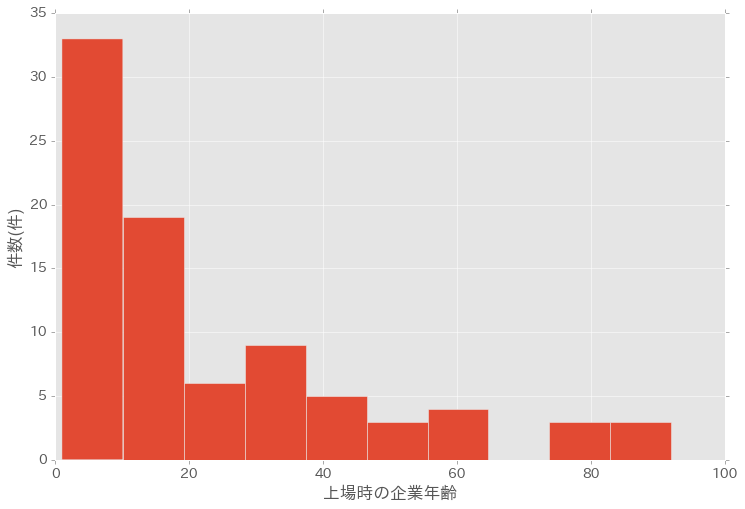
\includegraphics[clip,width=14cm]{./age.png}
    \label{agehist}
  \end{center}
\end{figure}

\begin{figure}[!h]
  \begin{center}
  \caption{IPO企業の上場時年齢の基本統計量の5年おきの推移(1997〜2016)}
\begin{tabular}{cccccc}
\hline
\  & 総計 & 1997 & 2002 & 2007 & 2012  \\
 \hline \hline
標準偏差 & 17.244 & 16.686 & 16.864 & 19.009 & 16.895   \\
\hline
平均値 & 22.724 & 25.480 & 21.295 & 24.671 & 19.613   \\
\hline
最小値 & 1 & 1 & 1 & 2 & 1   \\
25\% & 9 & 12 & 8 & 9 & 9   \\
50\% & 17 & 23 & 17 & 19 & 13   \\
75\% & 32 & 36 & 30 & 36 & 23   \\
最大値 & 97 & 96 & 92 & 97 & 90   \\
\hline
	\end{tabular}
	\label{age} 
  \end{center}
\end{figure}

\newpage

\subsubsection{上場時の企業年齢}
図\ref{agehist}と表\ref{age}に、IPO企業の、会社設立から上場までの所要年数を示した。中央値は16年と、比較的若い企業が多い。また、その構成は、年度の推移に関わらずほぼ一定であると言える。


\subsubsection{業種}
各企業は、日本証券コード委員会が定める、33業種が割り振られている。\par
業種ごとの上場企業数を示したものが表\ref{industry}である。IPOを行う企業の業種は、情報・通信業、卸売業、小売業、不動産業、サービス業などに偏っていることが分かる。

\subsubsection{主幹事証券会社}
主幹事とは、会社に代わって株式発行業務を引き受ける、幹事会社の代表のことである。公開株式の買取引受の他、ブックビルディング方式における公開価格の決定、IPOに際する社内管理体制の整備なども実施し、他のアンダーライターに比して、IPOに占める役割が大きい\footnote[11]{主幹事証券会社がアンダープライシングに与える影響を考察した研究は、国内でも盛んである。例えば、金子 (2009)\cite{kaneko}。}。\par
日本のIPO市場では、池田 (2010)\cite{ikeda2}が指摘するように、「どの年度も主幹事を務める証券会社はわずか20社程度で、大手証券会社3社(野村、大和、日興)の主幹事シェアが高い」(p.85) 。「米国における1980から1997年までの各年で主幹事を務めた証券会社(投資銀行)数は,最大で1997年の124社(IPO件数は407件)、最小で1989年と1990年の39社(IPO件数はそれぞれ108件、110件)である」(p.85)ことを考えると、日本におけるIPO主幹事の寡占度の高さが伺える。表\ref{lead}は、今回のサンプルにおける、主幹事上位5社のシェア(案件数ベース)である。\par

\subsubsection{上場市場}

いわゆる新興市場\footnote[12]{本稿では、JASDAQ(旧店頭市場、大証ヘラクレス、NEO含む)、マザーズ、福証Q-Board、札証アンビシャス、名証セントレックス。}と、通常の市場に上場する企業の数の年度別推移を図\ref{rising}に示す。 IPO数が伸びている時期は、主に新興市場での伸びが著しいと言えよう。

\newpage
\begin{table}[!h]
\centering

  \caption{証券コード協議会が定める33業種と本サンプルにおける件数}
\begin{tabular}{|c|c|c||c|c|c|}

\hline
番号 & 業種 & 件数 & 番号 & 業種 & 件数 \\
\hline \hline
1 & 水産・農林業 & 5 & 17 & 輸送用機器 & 15 \\
2 & 鉱業 & 3 & 18 & 精密機器 & 25 \\
3 & 建設業 & 57 & 19 & その他製品 & 51 \\
4 & 食料品 & 39 & 20 & 電気・ガス業 & 7 \\
5 & 繊維製品 & 4 & 21 & 陸運業 & 10 \\
6 & パルプ・紙 & 6 & 22 & 空運業 & 3 \\
7 & 化学 & 50 & 23 & 海運業 & 0 \\
8 & 医薬品 & 32 & 24 & 倉庫・運輸関連 & 14 \\
9 & 石油・石炭製品 & 2 & 25 & 情報・通信業 & 270 \\
10 & ゴム製品 & 1 & 26 & 卸売業 & 160 \\
11 & ガラス・土石製品 & 7 & 27 & 小売業 & 249 \\
12 & 鉄鋼 & 3 & 28 & 銀行業 & 11 \\
13 & 非鉄金属 & 9 & 29 & 証券・商品先物取引業  & 26 \\
14 & 金属製品 & 19 & 30 & 保険業 & 11 \\
15 & 機械 & 70 & 31 & その他金融業 & 26 \\
16 & 電気機器 & 96 & 32 & 不動産業 & 134 \\
17 & 輸送用機器 & 15 & 33 & サービス業 & 547 \\
18 & 精密機器 & 25 &  &  &  \\

\hline
	\end{tabular}
		\label{industry}
\end{table}

\begin{table}[h]
  \begin{center}
  \caption{主幹事上位5社のシェア(1997〜2016)}
\begin{tabular*}{120mm}{@{\extracolsep{\fill}}c|ccccc}

\hline
\ &  野村 &  大和 & 日興 & みずほ & SBI \\
\hline \hline
件数  &   536 & 399 & 293 & 74 & 35 \\
シェア & 27.3\% & 20.3\% & 14.9\% & 3.8\% & 1.8\% \\
\hline
	\end{tabular*}
	\label{lead} 
  \end{center}
\end{table}



\begin{figure}[!h]
  \begin{center}
  \caption{新興市場と非新興市場のIPO件数の推移(1997〜2016)}
    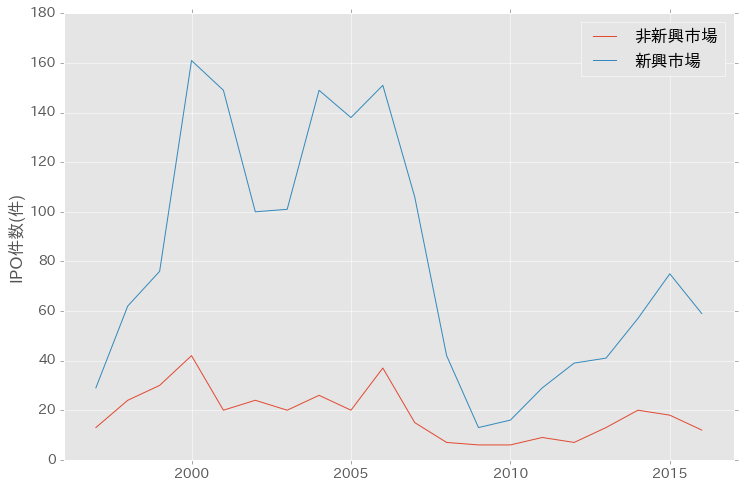
\includegraphics[clip,width=14cm]{./rising.png}
    \label{rising}
  \end{center}
\end{figure}

\newpage


\subsection{モデルの構造と想定される結果}
本稿では、「当該企業のIPOに対し、直近の数件のIPOのパフォーマンス自体がマーケット・コンディションとして影響している」という仮定を検証するために、アンダープライシングを被説明変数とする、p次の自己回帰モデルを用いる。パラメータは最小二乗法で推定し、AIC(赤池情報基準)から適切なラグ次数を算出する。\footnote[13]{なお、ソフトウェアとしてはPython 3.5.2、statsmodelsモジュールを用いた。ソースコードは\url{https://github.com/M-okb/IPO_analysis}で公開している。}\par
ここで、用いるデータ・セットは、各企業について、別々の一期間しか観測できない、アンバランスなパネルデータと解釈できる\footnote[14]{今回のサンプル・データには、期間内に上場廃止し、再上場を果たした企業は含まれていない。}。以下、添字tを以て、IPO企業を区別する。\\ \par
回帰式は次のようになる。\\ 
\begin{equation}
\label{reg}
\begin{split}
	UP_t = &\alpha + \beta_u ({\rm L}) UP_t + \beta_a Age_t + \beta_{int} Interval_t + \\
	 &\beta_m Market_t + \sum_{L} \beta_l Leader_t +  \sum_{I} \beta_{ind} Industry_t + \epsilon_t
\end{split}
\end{equation}
\newpage
ここで、$\beta_u({\rm L})$はラグ多項式であり、\par
\begin{equation}
\beta_u({\rm L}) = \sum_{i=1}^p \beta_{ui} {\rm L}^i \nonumber
\end{equation}\par
である。\\ \par


それぞれの変数について説明する。\\ \par
\begin{description}
 \item[$UP_t$]\mbox{}\\ 
 \{(初値) - (公開価格)\} / (公開価格)の自然対数を取ったもの。
  \item[$Age_t$]\mbox{}\\
  IPO企業のIPO時における企業年齢(年)の自然対数を取ったもの。若ければ若いほど、その企業についての情報量ギャップが大きいと考えられ、負の係数が予想される。
  \item[$Interval_t$]\mbox{}\\
  前回のIPOからの日数(日)。同日にIPOが実施される場合は、片方を0とした。マーケット・コンディション、すなわち$Underpricing$の程度が、公開企業のIPOの意思決定に影響を与えるなら、何らかの有意な値が想定される\footnote[15]{実際には、IPOの意思決定がなされるのは、上場する日の少なくとも1年以上前であり、また公開会社のキャッシュフローに直接影響を与えるのは、調達金額、すなわち公開価格$P_{book}$である。とは言え、東日本大震災や、リーマン・ショックなど、市況が悪化した際に、IPOを予定していた公開会社が上場延期を選択するケースは存在する。}。
  \item[$Market_t$]\mbox{}\\
  上場市場ダミー。上場先が新興市場のとき1を、それ以外で0を取る。新興市場の方が情報量ギャップが大きいと考えられ、正の係数が予想される。
  \item[$Leader_t$]\mbox{}\\
  主幹事ダミー群。それぞれ、シェア上位5位である、野村、大和、日興、みずほ、SBIであったときに1を、それ以外で0を取る。\\
  本稿では、主幹事の効果は時間を通して一定だと考えてモデルを組んでいる。もし、有意な正の係数が得られるならば、大手証券会社の寡占力\footnote[16]{金子 (2010)\cite{kaneko}は、主幹事の過小値付けの原因として3つの仮説を挙げている。中でも主幹事と公開会社の利益相反に着目した利益相反仮説では、「日本の総合証券会社のように,発行市場での引受業務のみならず流通市場での委託売買業務も営んでおり,しかも後者の方が主要な収入源である場合,新規公開企業の利益を犠牲にして大口投資家の利益を高める」と指摘している。利益相反仮説に立てば、寡占力の高さは価格決定力の高さだという前提の下、大手証券会社ダミーを説明変数に入れることで、利益相反仮説を検証できる。池田(2010)\cite{ikeda2}では、各証券会社ダミーと年度ダミーの交差項を説明変数に加え、年度ごとに効果を検証している。}の高さと解釈できる可能性がある。
  \item[$Industry_t$]\mbox{}\\
  業種ダミー群。各業種のときに1を、そうでないときに0を取る。完全な多重共線性を防ぐため、サービス業ダミーの取り除いている。すなわち、係数の意味はIPO企業がサービス業であった場合からのギャップである。情報通信業などの、新しいビジネス・モデルが起こりやすい業態において、正の係数が、金属製品などの素材産業で負の係数が予想される。\\ \\ 
\end{description}
  \par
また、IPOのマーケット・コンディションが、上場済みの株式市場とどういった関係にあるのかを把握するために、説明変数に当該IPO時における株式マーケットのインデックス\footnote[17]{日経平均株価 【998407】の日足終値を使用。単位は(円)。}を含めたモデルも推定する。\par
その場合の回帰式は、
\begin{equation}
\label{nikkeireg}
\begin{split}
	UP_t =  &\alpha + \beta_u (L) UP_t + \beta_a Age_t + \beta_v Interval_t + \\
	   &\beta_m Market_t + \sum_{K} \beta_l Leader_t +  \sum_{I} \beta_I Industry_t + \beta_n Nikkei_t+  \epsilon_t
\end{split}
\end{equation}

となる。\par


それぞれの変数間の相関係数を表\ref{corr}に示す。多重共線性の問題はないと考えられる。
\begin{table}[t]
  \begin{center}
  \caption{使用した各変数間の相関係数行列}
\begin{tabular}{c|cccccccccc}
\hline
 & $UP$ & $Nikkei$ & $Age$ & $Interval$ & $Market$ & $Nomura$ & $Daiwa$ & $Nikko$ & $Mizuho$ & $SBI$ \\
 \hline
$UP$ & 1.000 & &&&&&&&& \\
$Nikkei$ & 0.061 & 1.000 & &&&&&&& \\
$Age$ & -0.223 & 0.053 & 1.000 & &&&&&&  \\
$Interval$ & 0.045 & -0.090 & 0.000 & 1.000 & &&&&& \\
$Market$ & 0.235 & -0.049 & -0.259 & 0.005 & 1.000 & &&&& \\
$Nomura$ & -0.077 & 0.002 & 0.045 & 0.027 & -0.127 & 1.000 & &&& \\
$Daiwa$ & -0.007 & 0.022 & 0.045 & -0.045 & -0.100 & -0.309 & 1.000 & && \\
$Nikko$ & -0.003 & 0.070 & 0.025 & -0.030 & 0.009 & -0.256 & -0.211 & 1.000 &  &  \\
$Mizuho$ & -0.018 & 0.039 & 0.024 & 0.102 & 0.020 & -0.122 & -0.100 & -0.083 & 1.000 & \\
$SBI$ & 0.075 & 0.070 & -0.060 & 0.031 & 0.065 & -0.083 & -0.068 & -0.056 & -0.027 & 1.000 \\
\hline
	\end{tabular}
	\label{corr} 
  \end{center}
\end{table}
\par
$UP_t$の10次までの系列相関は、表\ref{autocorr}のようになっている。

\begin{table}[t]
  \begin{center}
  \caption{$UP_t$の系列相関}
\begin{tabular}{c|cccccccccc}
\hline
ラグ次数 & 0 & 1 & 2 & 3 & 4 & 5 & 6 & 7 & 8 & 9\\
系列相関 &1.000 & 0.326 & 0.335 & 0.293 & 0.278 & 0.272 & 0.242 & 0.239 & 0.211 & 0.236 \\
\hline \hline
ラグ次数 & 10 & 11 & 12 & 13 & 14 & 15 & 16 & 17 & 18 & 19 \\
系列相関 &0.248 & 0.240 & 0.197 & 0.192 & 0.217 & 0.198 & 0.203 & 0.174 & 0.179 & 0.170 \\
\hline
	\end{tabular}
	\label{autocorr} 
  \end{center}
\end{table}


\section{実証分析の結果}
実証分析の結果、回帰式(\ref{reg})、(\ref{nikkeireg})のいずれにおいても、$p = 15$が、AICを最小とするモデルとなった。\\ \par
表\ref{tab:reg}と表\ref{tab:regnikkei}に回帰分析の結果を示す。
また、図\ref{residual}が回帰式(\ref{reg})におけるOLS残差のプロットである。
\newpage

\begin{table}[h]
  \begin{center}
  \caption{回帰式(\ref{reg})の結果}
  \label{tab:reg}
\begin{tabular}{|c|ccccc|c|ccccc|}
\hline
 & 係数 & 標準誤差 & t値 & p値 &  &  & 係数 & 標準誤差 & t値 & p値 &  \\
 \hline\hline
定数項 & 0.1043 & 0.047 & 2.204 & 0.028 & ** & $industry_{1}$ & -0.0984 & 0.172 & -0.571 & 0.568 &  \\
$Age$ & -0.0651 & 0.012 & -5.591 & 0.000 & *** & $industry_{2}$ & -0.0258 & 0.223 & -0.116 & 0.908 &    \\
$Interval$ & 0.0037 & 0.001 & 3.215 & 0.001 & *** & $industry_{3}$ & -0.0547 & 0.055 & -0.998 & 0.318 &    \\
$Market$ & 0.2030 & 0.024 & 8.314 & 0.000 & *** & $industry_{4}$ & -0.1181 & 0.064 & -1.842 & 0.066 & *   \\
$Nomura$ & -0.0104 & 0.023 & -0.447 & 0.655 &  & $industry_{5}$ & -0.2161 & 0.193 & -1.122 & 0.262 &   \\
$Daiwa$ & 0.0325 & 0.025 & 1.290 & 0.197 &  & $industry_{6}$ & 0.0050 & 0.158 & 0.032 & 0.975 &   \\
$Nikko$ & 0.0136 & 0.028 & 0.493 & 0.622 &  & $industry_{7}$ & -0.0784 & 0.058 & -1.348 & 0.178 &    \\
$Mizuho$ & -0.1164 & 0.048 & -2.440 & 0.015 & ** & $industry_{8}$ & -0.2781 & 0.070 & -3.958 & 0.000 & ***   \\
$SBI$ & 0.0361 & 0.067 & 0.539 & 0.590 &  & $industry_{9}$ & -0.0958 & 0.271 & -0.354 & 0.724 &    \\
$UP_{t-1}$ & 0.1450 & 0.021 & 6.836 & 0.000 & *** & $industry_{10}$ & -0.0076 & 0.383 & -0.020 & 0.984 &   \\
$UP_{t-2}$ & 0.1496 & 0.021 & 6.972 & 0.000 & *** & $industry_{11}$ & 0.0527 & 0.147 & 0.359 & 0.719 &    \\
$UP_{t-3}$ & 0.0835 & 0.022 & 3.848 & 0.000 & *** & $industry_{12}$ & -0.2605 & 0.222 & -1.173 & 0.241 &    \\
$UP_{t-4}$ & 0.0500 & 0.022 & 2.305 & 0.021 & ** & $industry_{13}$ & -0.0535 & 0.129 & -0.414 & 0.679 &    \\
$UP_{t-5}$ & 0.0611 & 0.022 & 2.804 & 0.005 & *** & $industry_{14}$ & -0.2601 & 0.090 & -2.900 & 0.004 & ***   \\
$UP_{t-6}$ & 0.0199 & 0.022 & 0.915 & 0.360 &  & $industry_{15}$ & -0.1210 & 0.050 & -2.427 & 0.015 & **   \\
$UP_{t-7}$ & 0.0340 & 0.022 & 1.561 & 0.119 &  & $industry_{16}$ & 0.0036 & 0.043 & 0.084 & 0.933 &    \\
$UP_{t-8}$ & 0.0202 & 0.022 & 0.925 & 0.355 &  & $industry_{17}$ & -0.1719 & 0.112 & -1.537 & 0.125 &    \\
$UP_{t-9}$ & 0.0357 & 0.022 & 1.641 & 0.101 &  & $industry_{18}$ & -0.0721 & 0.079 & -0.917 & 0.359 &  \\
$UP_{t-10}$ & 0.0655 & 0.022 & 3.010 & 0.003 & ** & $industry_{19}$ & -0.0842 & 0.057 & -1.477 & 0.140 &   \\
$UP_{t-11}$ & 0.0349 & 0.022 & 1.607 & 0.108 &  & $industry_{20}$ & 0.0425 & 0.146 & 0.291 & 0.771 &   \\
$UP_{t-12}$ & -0.0080 & 0.022 & -0.369 & 0.712 &  & $industry_{21}$ & -0.0882 & 0.123 & -0.715 & 0.474 &   \\
$UP_{t-13}$ & -0.0088 & 0.022 & -0.404 & 0.686 &  & $industry_{22}$ & -0.0341 & 0.222 & -0.154 & 0.878 &   \\
$UP_{t-14}$ & 0.0476 & 0.021 & 2.218 & 0.027 & ** & $industry_{24}$ & -0.0291 & 0.104 & -0.280 & 0.779 &   \\
$UP_{t-15}$ & 0.0329 & 0.021 & 1.541 & 0.123 &  & $industry_{25}$ & 0.2132 & 0.029 & 7.374 & 0.000 & ***   \\
\cline{1-6}
\multicolumn{3}{|c|}{Adjusted $R^2$} &\multicolumn{3}{|c|}{0.334} & $industry_{26}$ & -0.0217 & 0.035 & -0.620 & 0.535 &    \\
\multicolumn{3}{|c|}{F統計量} &\multicolumn{3}{|c|} {19.07}  & $industry_{27}$ & -0.0889 & 0.030 & -3.010 & 0.003 & ***  \\
\multicolumn{3}{|c|}{AIC} &\multicolumn{3}{|c|} {1816}   & $industry_{28}$ & -0.0616 & 0.118 & -0.523 & 0.601 &    \\
\multicolumn{3}{|c|}{BIC}&\multicolumn{3}{|c|} {2123} & $industry_{29}$ & -0.1515 & 0.077 & -1.973 & 0.049 & **   \\
\multicolumn{3}{|c|}{DW比} &\multicolumn{3}{|c|}{1.939} &   $industry_{30}$ & 0.0623 & 0.117 & 0.532 & 0.595 &    \\
\multicolumn{3}{|c|}{サンプル数} &\multicolumn{3}{|c|}{1947}  & $industry_{31}$ & -0.0298 & 0.077 & -0.385 & 0.700 &    \\
\cline{1-6}
\multicolumn{3}{|c|}{} &\multicolumn{3}{|c|}{}  & $industry_{32}$ & -0.0342 & 0.037 & -0.922 & 0.357 &    \\
\hline
	\end{tabular}
  \end{center}
\end{table}

\newpage



\begin{table}[h]
  \begin{center}
  \caption{回帰式(\ref{nikkeireg})の結果}
  \label{tab:regnikkei}
\begin{tabular}{|c|ccccc|c|ccccc|}
\hline
 & 係数 & 標準誤差 & t値 & p値 &  &  & 係数 & 標準誤差 & t値 & p値 &  \\
 \hline\hline
定数項 & 0.0588 & 0.058 & 1.005 & 0.315 &  & $industry_{1}$ & -0.0993 & 0.172 & -0.576 & 0.565 &  \\
$Age$ & -0.0656 & 0.012 & -5.635 & 0 & *** & $industry_{2}$ & -0.0134 & 0.223 & -0.06 & 0.952 &  \\
$Interval$ & 0.0038 & 0.001 & 3.316 & 0.001 & *** & $industry_{3}$ & -0.0588 & 0.055 & -1.072 & 0.284 &  \\
$Market$ & 0.204 & 0.024 & 8.352 & 0 & *** & $industry_{4}$ & -0.1177 & 0.064 & -1.836 & 0.066 & * \\
$Nomura$ & -0.0124 & 0.023 & -0.53 & 0.596 &  & $industry_{5}$ & -0.2089 & 0.193 & -1.084 & 0.278 &  \\
$Daiwa$ & 0.03 & 0.025 & 1.185 & 0.236 &  & $industry_{6}$ & 0.0084 & 0.158 & 0.053 & 0.958 &  \\
$Nikko$ & 0.0097 & 0.028 & 0.351 & 0.725 &  & $industry_{7}$ & -0.0785 & 0.058 & -1.351 & 0.177 &  \\
$Mizuho$ & -0.121 & 0.048 & -2.53 & 0.011 & ** & $industry_{8}$ & -0.2751 & 0.07 & -3.915 & 0 & *** \\
$SBI$ & 0.0284 & 0.067 & 0.423 & 0.672 &  & $industry_{9}$ & -0.0945 & 0.271 & -0.349 & 0.727 &  \\
$UP_{t-1}$ & 0.1446 & 0.021 & 6.819 & 0 & *** & $industry_{10}$ & -0.0073 & 0.382 & -0.019 & 0.985 &  \\
$UP_{t-2}$ & 0.1491 & 0.021 & 6.949 & 0 & *** & $industry_{11}$ & 0.0539 & 0.147 & 0.368 & 0.713 &  \\
$UP_{t-3}$ & 0.0832 & 0.022 & 3.834 & 0 & *** & $industry_{12}$ & -0.2619 & 0.222 & -1.18 & 0.238 &  \\
$UP_{t-4}$ & 0.0499 & 0.022 & 2.304 & 0.021 & ** & $industry_{13}$ & -0.0571 & 0.129 & -0.441 & 0.659 &  \\
$UP_{t-5}$ & 0.0608 & 0.022 & 2.791 & 0.005 & *** & $industry_{14}$ & -0.2623 & 0.09 & -2.925 & 0.003 & *** \\
$UP_{t-6}$ & 0.0196 & 0.022 & 0.9 & 0.368 &  & $industry_{15}$ & -0.1241 & 0.05 & -2.486 & 0.013 & ** \\
$UP_{t-7}$ & 0.0337 & 0.022 & 1.548 & 0.122 &  & $industry_{16}$ & 0.0056 & 0.043 & 0.131 & 0.896 &  \\
$UP_{t-8}$ & 0.0199 & 0.022 & 0.912 & 0.362 &  & $industry_{17}$ & -0.1715 & 0.112 & -1.533 & 0.125 &  \\
$UP_{t-9}$ & 0.0354 & 0.022 & 1.625 & 0.104 &  & $industry_{18}$ & -0.0705 & 0.079 & -0.897 & 0.37 &  \\
$UP_{t-10}$ & 0.0652 & 0.022 & 3.001 & 0.003 & ** & $industry_{19}$ & -0.085 & 0.057 & -1.489 & 0.137 &  \\
$UP_{t-11}$ & 0.0345 & 0.022 & 1.588 & 0.112 &  & $industry_{20}$ & 0.044 & 0.146 & 0.301 & 0.763 &  \\
$UP_{t-12}$ & -0.0084 & 0.022 & -0.385 & 0.7 &  & $industry_{21}$ & -0.0877 & 0.123 & -0.711 & 0.477 &  \\
$UP_{t-13}$ & -0.0093 & 0.022 & -0.427 & 0.669 &  & $industry_{22}$ & -0.0267 & 0.222 & -0.121 & 0.904 &  \\
$UP_{t-14}$ & 0.0471 & 0.021 & 2.193 & 0.028 & ** & $industry_{24}$ & -0.0268 & 0.104 & -0.258 & 0.796 &  \\
$UP_{t-15}$ & 0.0321 & 0.021 & 1.503 & 0.133 &  & $industry_{25}$ & 0.2119 & 0.029 & 7.326 & 0 & *** \\
$Nikkei$ & 0 & 0.0000 & 1.326 & 0.185 &  & $industry_{26}$ & -0.0206 & 0.035 & -0.589 & 0.556 &  \\
\cline{1-6}
\multicolumn{3}{|c|}{Adjusted $R^2$} &\multicolumn{3}{|c|}{0.334} & $industry_{27}$ & -0.0901 & 0.03 & -3.049 & 0.002 & *** \\
\multicolumn{3}{|c|}{F統計量} &\multicolumn{3}{|c|}{18.76} & $industry_{28}$ & -0.063 & 0.118 & -0.535 & 0.593 &  \\
\multicolumn{3}{|c|}{AIC} &\multicolumn{3}{|c|}{1817}& $industry_{29}$ & -0.1513 & 0.077 & -1.971 & 0.049 & ** \\
\multicolumn{3}{|c|}{BIC} &\multicolumn{3}{|c|}{2129} &$industry_{30}$ & 0.0651 & 0.117 & 0.556 & 0.578 &  \\
\multicolumn{3}{|c|}{DW比} &\multicolumn{3}{|c|}{1.94} & $industry_{31}$ & -0.0282 & 0.077 & -0.365 & 0.715 &  \\
\multicolumn{3}{|c|}{サンプル数} &\multicolumn{3}{|c|}{ 1947} & $industry_{32}$ & -0.0331 & 0.037 & -0.892 & 0.372 &  \\
\hline
	\end{tabular}
  \end{center}
\end{table}
\newpage

\begin{figure}[!t]
  \begin{center}
  \caption{回帰式(1)における残差のプロット}
    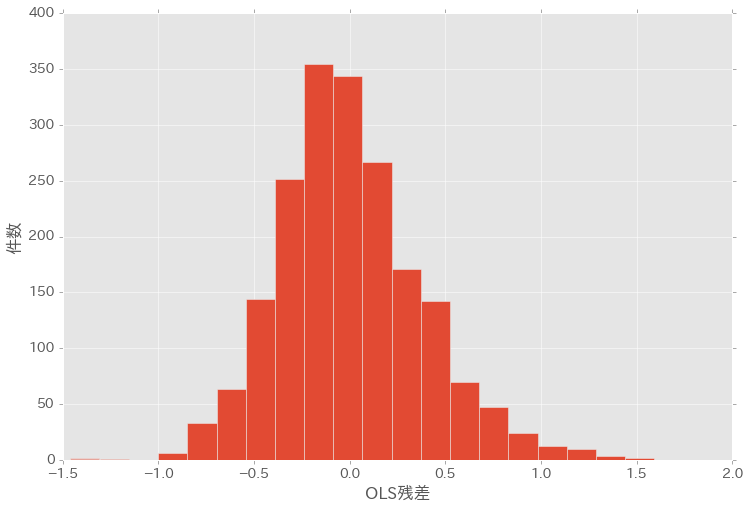
\includegraphics[clip,width=14cm]{./residual.png}
    \label{residual}
  \end{center}
\end{figure}
\par
アンダープライシングのラグ項$\beta_u({\rm L})UP_t$は、特に5次の項までの係数の推定値も比較的大きく、有意な値が続いている。「直近のIPOのパフォーマンス自体がアンダープライシングの度合いに影響する」という仮説を検証したと言えるだろう。\par
企業年齢や、上場市場ダミーについても、想定通りの有意な値が得られた。「情報量ギャップが大きいほど、アンダープライシングは大きくなる」という仮説と整合的である。\par
業種ダミーについては、「食料品」「医薬品」「金属製品」「機械」「小売」「商品先物取引」で負の、「情報通信業」で正の有意な係数が得られた。これもほぼ想定通りである。\\ \par
主幹事ダミーについては、みずほ証券\footnote[18]{新光証券と合併する前の、旧みずほ証券の発足が2000年であり、当然、今回のサンプル・データにおいても、みずほ証券は2000年以降しか主幹事を務めていない。しかし、2000年以前と以後でアンダープライシングの度合いに大きな差がない(図\ref{transition}参照)こと、本サンプルにおいてSBI証券の主幹事が始まったのも2010年からであることなどから、取扱年度が関係しているとは断言できない。}のみ、負の有意な値が得られた。今回のデータだけでは、「みずほ証券は公開価格を適正に判断している」のか「みずほ証券が主幹事を務める企業に、アンダープライシングを押し下げる要因がある」のか判断が出来ないが、興味深い結果ではある。いずれにせよ、利益相反仮説と整合的な結果は得られなかった。\par
日経平均株価は、有意な係数を得られず、推定された係数も非常に小さいものだった。AICも、わずかながら$Nikkei$を説明変数に加えない式(\ref{reg})の方が、小さい値を示した。この実験だけから断言することは出来ないが、「アンダープライシングというマーケットが、通常の株式市場と強い関係を持たないこと」を示唆すると考える。\par

IPO間隔については、「IPO頻度はマーケット・コンディションと負の相関を持つ」ことを示唆する有意な結果が得られた。\\ \par
これは、少し意外な結果である。どのように解釈すればよいのだろうか?\\ \par
一つの仮説であるが、通常、IPOの日程は種々の理由\footnote[19]{例えば、会計・簿記上の都合や、証券会社の業務上の都合など。}から一定の日にちに集中しやすいのだが、アンダープライシングが発生しやすいような企業は、その制約から外れやすく\footnote[20]{新規サービスゆえ、証券会社の監査が延長される、公開会社が高いプライシングを期待しており、証券会社と揉めやすい、など。}、結果、IPO間隔が伸びやすい、というようなことは考えられる。\par
とは言え、この仮説の検証には、本稿では力不足である。むしろ、ブックビルディングによる公開価格$P_{book}$の決定プロセスや、IPO間隔でなく、IPOの日別の集中度のリサーチ、証券会社へのヒアリングが必要になるだろう。

図\ref{interval}はIPO間隔とアンダープライシングをプロットしたものである。\par

\begin{figure}[!t]
  \begin{center}
  \caption{IPOの間隔(横軸)と、アンダープライシング(縦軸、対数)の散布図。破線は、アンダープライシングの平均値}
    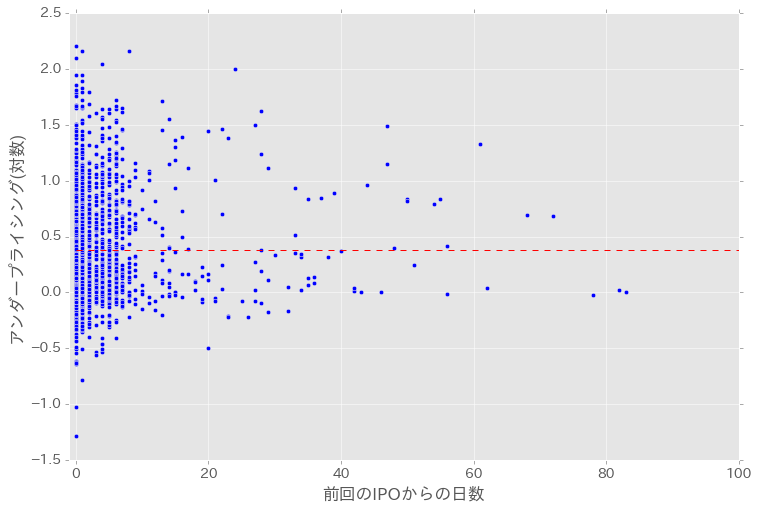
\includegraphics[clip,width=14cm]{./interval.png}
    \label{interval}
  \end{center}
\end{figure}

\newpage
\section{総括と今後の課題}
本稿では、「当該企業のIPOに対し、直近の数件のIPOのパフォーマンス自体がマーケット・コンディションとして影響している」という仮説を検証し、実証分析の結果、おおむね仮説を裏付ける結果を得た。\par
また、「IPOにおけるマーケット・コンディションは、日経平均株価とは関係がない」という結果も暗示された。とは言え、マーケットの独立性を、高い説得力を以て主張するためには、今後の更なる工夫と検証を要する。\par
企業年齢・上場市場ダミー・業種ダミーについては、当初の想定通り、「投資家に情報量が不足しているほど、アンダープライシングが大きくなる」という結果が得られた。\par
一方で、主幹事ダミーについては、みずほ証券のみ有意な負の係数が推定された。池田(2010)\cite{ikeda2}においても、2004年以降は利益相反仮説を示す有意な証拠は得られていなかった。年度を通して変化する環境\footnote[21]{池田(2010)\cite{ikeda2}では、銀行系証券会社の参入による競争激化を挙げている。}が存在するなら、主幹事の影響を年度ごとに変化する値としてモデルを組み直し、検証されるべきだろう。\par
IPOの間隔については、有意な負の値が得られた。前頁で1つの仮説を述べたが、IPOの集中度がアンダープライシングに与える影響については、更なる仮説の提示・実証分析による検証が待たれる。\\ \par

さて、最後にブックビルディングによる公開価格の決定方法について、問題を提起したい。\par
本稿を通して、$P_{open}$がマーケット・コンディションによって大きく変動することを指摘してきた。その$P_{book}$との乖離は、そのまま公開会社の資金調達における機会損失なのであるから、$P_{book}$はファンダメンタルズ・バリューに固執し過ぎるのでなく、過去のアンダープライシングなどの、マーケット・コンディションを考慮して、決定されるべきである。\\ \par
本稿が、より効率的なIPO市場に貢献できれば幸いである。


\newpage


\begin{thebibliography}{99}
\bibitem{ikeda} 池田直史 (2013) 「IPOの株価観察不能性と正の初期収益率」, 『金融経済研究, 第35号 34-51』
\bibitem{ikeda2} 池田直史 (2010) 「IPOにおける大手証券会社の引受と初期収益率:利益相反仮説の検証」, 『三田商学研究 第53巻 第1号』
\bibitem{okamura} 岡村秀夫 (2011)「IPO研究の展開」, 『商学論究, 58(3):45-65』
\bibitem{kaneko} 金子隆 (2009) 「IPOの過小値付け現象 −新しい解釈の試み−」, 『三田商学研究 第52巻 第2号』
\bibitem{tatsumi} 辰巳憲一・桂山靖代 (2005)「IPOリターン・リバーバル —初取引日前後IPOパフォーマンスのアノマリー分析—」, 『学習院大学 経済論集, 第42巻 第3号』
\bibitem{Derrien} Derrien, F. (2005) "IPO Pricing in "Hot" Market Conditions: Who Leaves Money On the Table?," Journal of Finance 60, 487-615
\bibitem{Loughran} Loughram, T., Ritter, J. and Rydqvist, K. (1994) "Initial Public Offering: International Insights," Pacific-Basin Finance Journal 2, 165-199. (updated 2015)
\bibitem{Welch} Welch, I. (1992) "Sequential Sales, Learning, and Cascades," The Journal of FINANCE 47, 695-732.

\end{thebibliography}

\end{document}